\documentclass{report}
\usepackage{ugentstyle}

\newcommand{\answer}[1]{
		\subsubsection*{Antwoord}
			#1
}

\begin{document}
	\maketitle{Compilers - Voorbeeldexamen}
	\tableofcontents
	\chapter{Vragen}
	\section{Compilerfasen - I}
	Gegeven de opeenvolgende fasen van een compiler, geef aan de programmavoorstellingen, grafen of datastructuren die aan het \textit{eind} van elke fase geproduceerd worden. Geef uw antwoord in de vorm: a-7, b-3, ...
	\begin{table}[ht]
		\begin{tabular}{l l}
			\hline
			Compilerfase & Programmavoorstelling \\
			\hline 
			(a) scanning (lexicale analyse) & 1.  intermediaire boomtaal \\
			(b) parsing  (syntactische analyse) & 2.  control flow graaf (CFG) \\
			(c) type checking (semantische analyse) & 3.  frame layout, activation records \\
			(d) vertaling (translate) & 4.  symbooltabellen \\
			(e) canonicalisering & 5.  interferentiegraaf \\
			(f) instructieselectie & 6.  gekleurde interference graph \\
			(g) controlestroom analyse & 7.  tokens \\
			(h) dataflow analyse (liveness) & 8.  assembler code \\
			(i) register allocatie & 9.  assembler instructies \\
			(j) code emission & 10.  abstracte syntax tree (AST)
		\end{tabular}
	\end{table}

	\answer{a-7, b-10, c-?, d-?, e-?, f-9, g-?, h-6, i-?, j-8}

	\newpage
	\section{Lexicale analyse}
	\label{sec:lexicale_analyse}
	
	Volgende nondeterministische eindige automaat herkent geldige tokens \texttt{(aa)+} en \texttt{(aaa)+}. 
	\begin{figure}[ht]
		\centering
		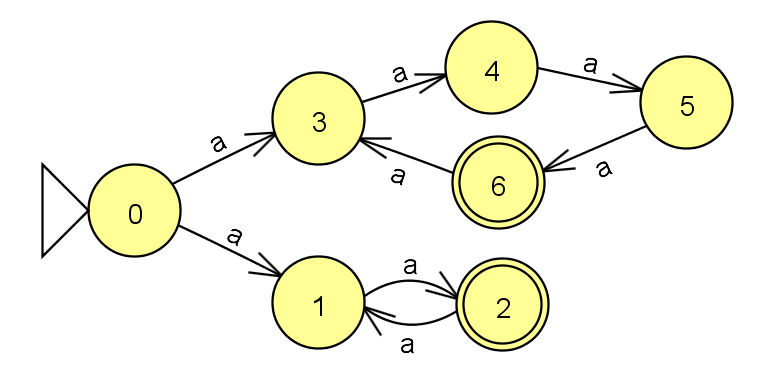
\includegraphics[width=\textwidth]{vr2_niet_deterministische_automaat}
	\end{figure}
	\begin{enumerate}
		\item Beschrijf de manier om in het algemeen verschillende NFA's samen te voegen tot 1 DFA. Bespreek daarbij de definitie van \textit{sluiting}, \textit{DFAedge} en het \textit{algoritme} dat de NFA-toestanden samenvoegt tot toestanden in een DFA.
		\item Pas dit toe op dit voorbeeld: de herkenning van twee- en drievouden van \texttt{a} en teken de bekomen DFA.
		\item Zijn er in de gevonden DFA nog equivalente toestanden die men kan vereenvoudigen?
	\end{enumerate}

	\answer{
	\begin{enumerate}
		\item Een deterministische eindige automaat (DFA) is een eindige automaat waarbij elke transitie uniek is. Het algoritme om een NFA om te vormen naar een DFA maakt enerzijds gebruik van sluitingen. De sluiting $T$ van een verzameling van toestanden $S$, of \texttt{closure(S)}, bevat alle toestanden die kunnen bereikt worden voor de lege transitie $\epsilon$ voor elke staat in $S$. Dit kan wiskundig gedefinieerd worden als:
		$$T = S \cup \bigg(\bigcup_{s \in T} edge(s, \epsilon) \bigg)$$
		waarbij \texttt{edge(s, c)} de staten geeft die vanuit $s$ via symbool $c$ kan bereikt worden.
		
		Anderzijds maakt het algoritme ook gebruik van de functie \texttt{DFAedge(d, c)}, die de staten teruggeeft die vanuit $d$ kunnen bereikt worden bij symbool $c$.
		
		\todo{verder uitleggen}
		
		\item De automaat is enkel in staat om enkelvoudige $a$ symbolen te verwerken en aangezien er geen lege strings zijn, draagt de \texttt{closure(S)} functie hier niets bij. De eerste verwerking zorgt ervoor dat staten 1 en 3 bereikt worden. Vanuit 1 kan er naar 2 gegaan worden en vanuit 3 kan er naar 4 gegaan worden. In dit geval moet dit herhaald worden tot dat er een combinatie van staten gevonden is die al eerder gecombineerd zijn. Dit is het geval als uiteindelijk de staten 6 en 2 bereikt worden. Vanuit 6 kan naar 3 gegaan worden en vanuit 2 kan naar 1 gegaan worden. Die combinatie bestaat al, en da DFA is voltooid.
			
		\begin{figure}[ht]
			\centering
			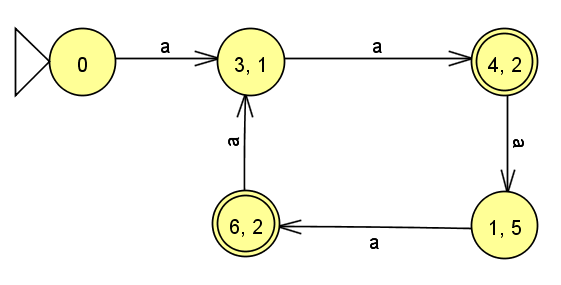
\includegraphics[width=\textwidth]{vr2_deterministische_automaat}
		\end{figure}
	
		\item Het algoritme garandeerd niet dat de opgeleverde DFA optimaal is, maar er kunnen nadien wel nog optimalisaties doorgevoerd worden. Staten die equivalent zijn kunnen samengenomen worden. Een staat $s_1$ is equivalent met staat $s_2$ als ze beiden finaal of niet finaal zijn voor dezelfde symbolen en als voor elk symbool $c$, trans[$s_1, c$] = trans[$s_1, c$]. In dit geval is dit waar voor staat $\{3, 1\}$ met $\{1, 5\}$ en voor staat $\{4, 2\}$ met $\{6, 2\}$. Deze kunnen gecombineerd worden.
		
		\begin{figure}[ht]
			\centering
			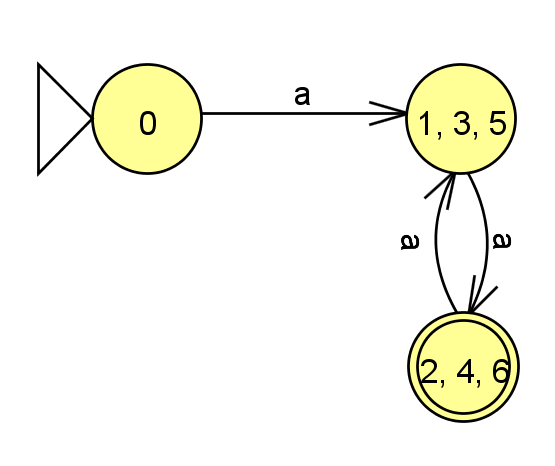
\includegraphics[width=\textwidth]{vr2_deterministische_automaat_minified}
		\end{figure}
		
		
	\end{enumerate}	
}

	\newpage
	\section{Compilerfasen - II}
	
	De volgende figuur toont de intermediaire voorstellingen die gebruikt worden als interface tussen de verschillende fasen van een compiler. Vul de nummers in van de corresponderende fasen in een compiler.
	\begin{figure}[ht]
		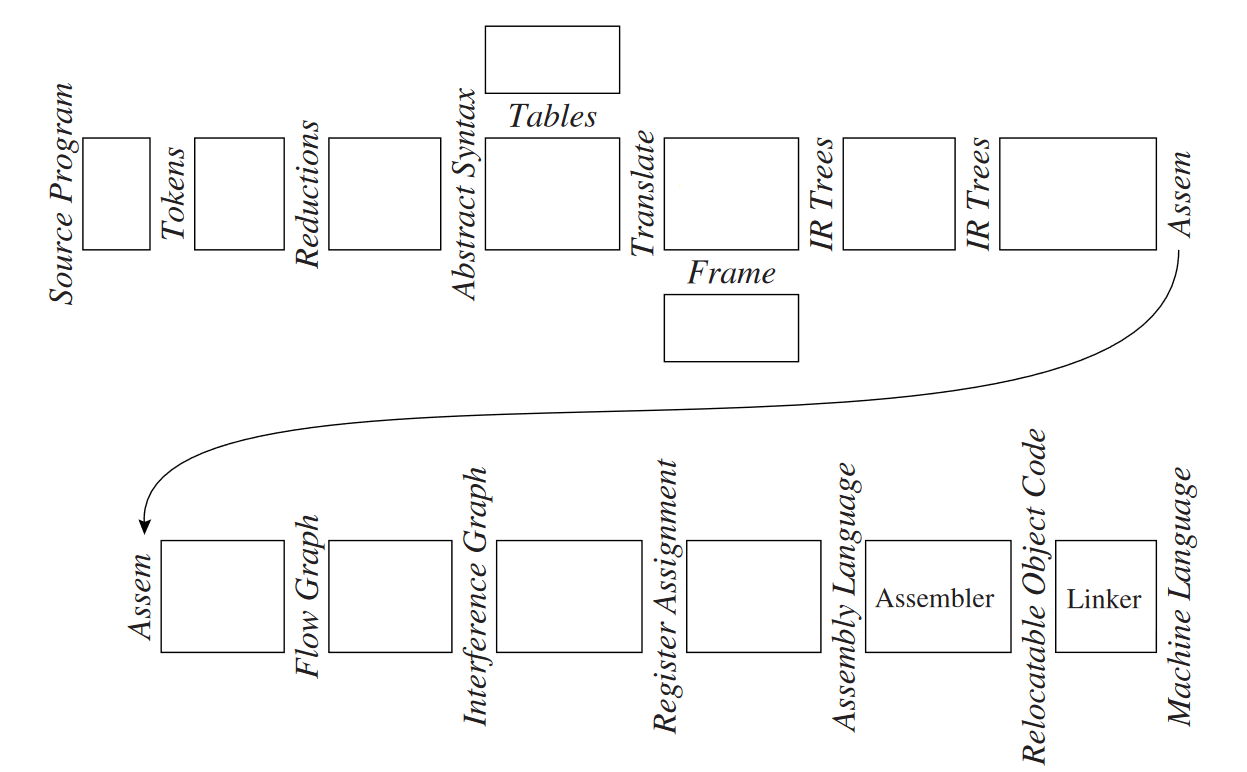
\includegraphics[width=\textwidth]{compiler_fasen}
	\end{figure}
	\begin{enumerate}
		\item Canonicalize
		\item Code Emission
		\item Control Flow Analysis
		\item Data Flow Analysis
		\item Environments
		\item Frame Layout
		\item Instruction Selection
		\item Lex
		\item Parse
		\item Parsing Actions
		\item Register Allocation
		\item Semantic Analysis
		\item Translate
	\end{enumerate}
	\answer{
		\begin{figure}[ht]
			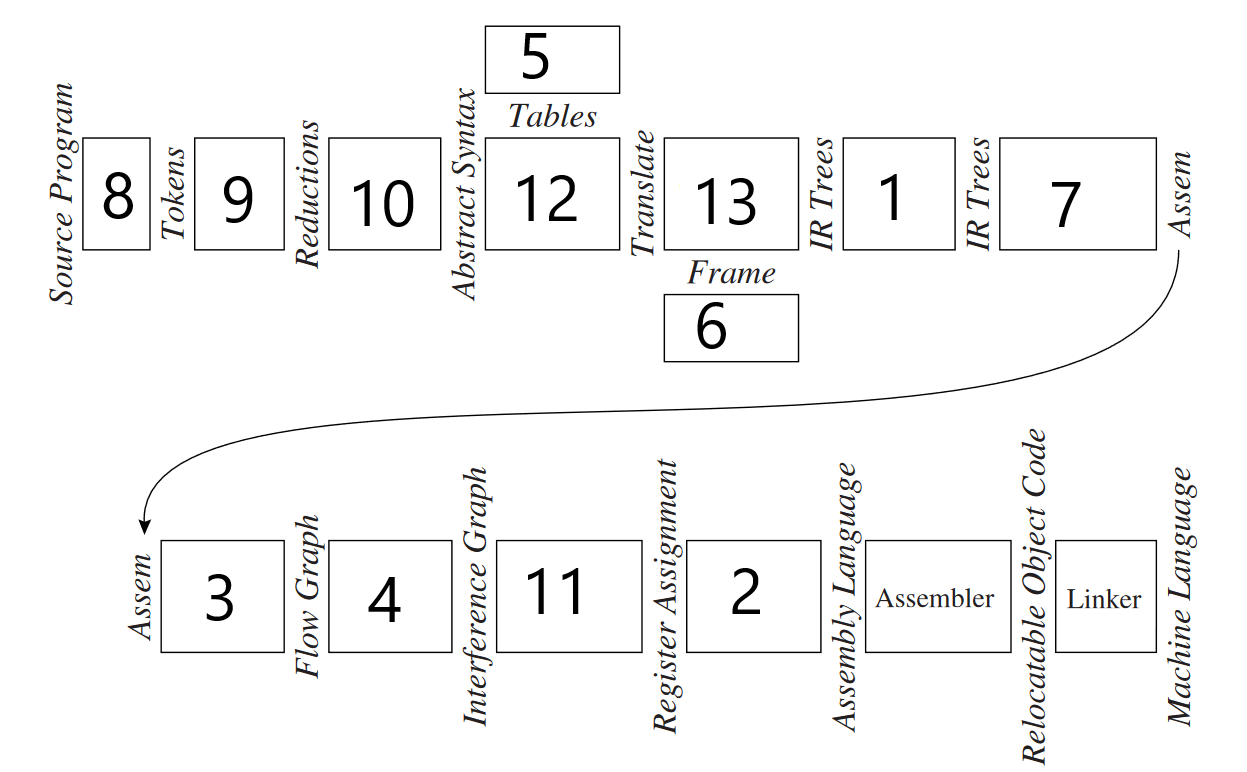
\includegraphics[width=\textwidth]{compiler_fasen_solved}
		\end{figure}
	}

	\newpage
	\section{NFA}
	\begin{figure}[ht]
		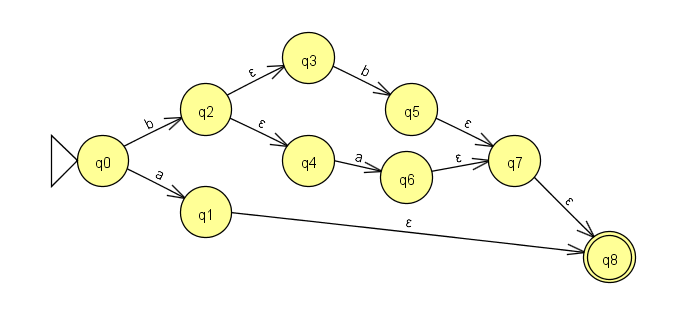
\includegraphics[width=\textwidth]{vr4_niet_deterministische_automaat}
	\end{figure}
	\begin{enumerate}
		\item Converteer deze NFA naar een DFA.
		\item Welke reguliere expressie wordt hiermee voorgesteld?
	\end{enumerate}
	\answer{
		\begin{enumerate}
			\item Gebruik dezelfde methodologie als in vraag \ref{sec:lexicale_analyse}.	\begin{figure}[ht]
				\centering
				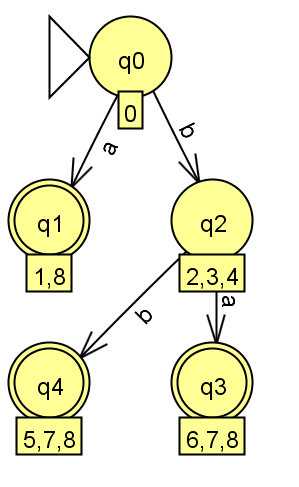
\includegraphics[width=0.5\textwidth]{vr4_deterministische_automaat}
			\end{figure}
		\item De reguliere expressie die voorgesteld wordt is $$\texttt{a+ba+bb}$$
		\todo{hoe bekomen}
		\end{enumerate}
	}

	\newpage
	\section{Parsing - I}
	Gegeven de grammatica
	\begin{align*}
	S & \mapsto E \\
	E & \mapsto E + T \\
	E & \mapsto T \\
	T & \mapsto F \\
	F & \mapsto a \\
	F & \mapsto b
	\end{align*}

	\begin{enumerate}
		\item Welke zijn de items in de initiële toestand (1) van de LR(0) parser generator?
		\item Teken de toestanden die bereikt worden na één shift of reduce actie van de LR(0) parser generator vanuit toestand 1. Teken ook de items in elke toestand.
	\end{enumerate}
	\answer{
		\begin{enumerate}
			\item 	Elke productieregel wordt een item in deze initiële toestand voor deze grammaatica.
			\begin{figure}[ht]
				\centering
				\begin{tikzpicture}[state/.style={rectangle, draw, inner sep = 2mm}]
				\node (1) [state] {
					$\begin{aligned}
					S & \mapsto .E \\
					E & \mapsto .E + T \\
					E & \mapsto .T \\
					T & \mapsto .F \\
					F & \mapsto .a \\
					F & \mapsto .b
					\end{aligned}$};
				\node (label1) [anchor=north east, inner sep = 1pt] at (1.north east) {\textbf{1.}};
				\end{tikzpicture}
			\end{figure}
			\item Vanuit de eerste toestand zijn er enkel shift acties mogelijk. 
			\begin{figure}[ht]
				\centering
				\begin{tikzpicture}[state/.style={rectangle, draw, inner sep = 2mm}]
				\node (1) [state] {
					$\begin{aligned}
					S & \mapsto .E \\
					E & \mapsto .E + T \\
					E & \mapsto .T \\
					T & \mapsto .F \\
					F & \mapsto .a \\
					F & \mapsto .b
					\end{aligned}$};
				
			\node (2) [state, above = 1.5cm of 1] {$
				\begin{aligned}
					S & \mapsto E. \\
					E & \mapsto E. + T \\
				\end{aligned}
				$};
			\node (3) [state, right = 1.5cm of 1] {$
				\begin{aligned}
				E & \mapsto T. \\
				\end{aligned}
				$};
			\node (4) [state, below = 1.5cm of 3] {$
				\begin{aligned}
				T & \mapsto F. \\
				\end{aligned}
				$};
			
			\node (5) [state, left = 1.5cm of 1] {$
				\begin{aligned}
				F & \mapsto a. \\
				\end{aligned}
				$};
			\node (6) [state, below = 1.5cm of 5] {$
				\begin{aligned}
				F & \mapsto b. \\
				\end{aligned}
				$};
			
			
			
			
			\draw [->] (1) -- node[xshift=0.25cm] {E} (2);
			\draw [->] (1) -- node[yshift=0.25cm] {T} (3);
			\draw [->] (1) -- node[yshift=0.25cm] {F} (4);
			\draw [->] (1) -- node[yshift=0.25cm] {a} (5);
			\draw [->] (1) -- node[yshift=0.25cm] {b} (6);
			
			\node (label1) [anchor=north east, inner sep = 1pt] at (1.north east) {\textbf{1.}};
			\node (label2) [anchor=north east, inner sep = 1pt] at (2.north east) {\textbf{2.}};
			
			\node (label3) [anchor=north east, inner sep = 1pt] at (3.north east) {\textbf{3.}};
			\node (label4) [anchor=north east, inner sep = 1pt] at (4.north east) {\textbf{4.}};
						
			\node (label5) [anchor=north east, inner sep = 1pt] at (5.north east) {\textbf{5.}};
			\node (label6) [anchor=north east, inner sep = 1pt] at (6.north east) {\textbf{6.}};

			\end{tikzpicture}
		\end{figure}
	\end{enumerate}}
	
	\newpage
	\section{Parsing - II}
	Gegeven de volgende context-vrije grammatica:
	
	\centering
	\begin{minipage}{0.5\textwidth}
		\begin{enumerate}
			\item[0.] $S  \mapsto E\$$
			\item[1.] $E  \mapsto id$
			\item[2.] $E  \mapsto id(E)$
			\item[3.] $E  \mapsto E + id$
		\end{enumerate}
	\end{minipage}

	\begin{enumerate}
		\item Bouw een LR(0) DFA voor deze grammatica.
		\item Is dit een LR(0) grammatica? Toon aan Waarom.
		\item Is dit een SLR grammatica? Toon aan Waarom.
		\item Is dit een LR(1) grammatica? Toon aan Waarom.
	\end{enumerate}
	\answer{
		\begin{enumerate}
			\item De LR(0) toestandenautomaat:
			
				\begin{figure}[ht]
				\centering
				\begin{tikzpicture}[state/.style={rectangle, draw, inner sep = 2mm}]
				\node (1) [state] {
					$\begin{aligned}
						S & \mapsto .E\$ \\
						E & \mapsto .id\\
						E & \mapsto .id(E) \\
						E & \mapsto .E + id
					\end{aligned}$};
				
				\node (2) [state, right = 1.5cm of 1] {$
					\begin{aligned}
					S & \mapsto E.\$ \\
					E & \mapsto E. + id\\
					\end{aligned}
					$};
				
				\node (3) [state, below = 1.5cm of 2] {$
					\begin{aligned}
					E & \mapsto E+.id \\
					\end{aligned}
					$};
				\node (4) [state, right = 1.5cm of 3] {$
					\begin{aligned}
					E & \mapsto E+id. \\
					\end{aligned}
					$};
				
				\node (5) [state, below = 1.5cm of 1] {$
					\begin{aligned}
					E & \mapsto id. \\
					E & \mapsto id.(E) \\
					\end{aligned}
					$};
				
				\node (6) [state, below = 1.5cm of 5] {$
					\begin{aligned}
					E & \mapsto id(.E) \\
					E & \mapsto .id \\
					E & \mapsto .id(E) \\
					E & \mapsto .E + id
					\end{aligned}
					$};
			   \node (7) [state, right = 1.5cm of 6] {$
					\begin{aligned}
					E & \mapsto id(E.) \\
					E & \mapsto E. + id
					\end{aligned}
					$};
				
				\node (8) [state, right = 1.5cm of 7] {$
					\begin{aligned}
					E & \mapsto id(E). \\
					\end{aligned}
					$};
				
				\draw [->] (1) -- node[yshift=0.25cm] {E} (2);
				\draw [->] (2) -- node[xshift=0.25cm] {+} (3);
				\draw [->] (3) -- node[yshift=0.25cm] {id} (4);
				\draw [->] (1) -- node[xshift=0.25cm] {id} (5);
				\draw [->] ([xshift=-20pt] 5.south) -- node[xshift=-0.5cm] {(} ([xshift=-20pt] 6.north);
				\draw [->] ([xshift=20pt] 6.north) -- node[xshift=0.5cm] {id} ([xshift=20pt] 5.south);
				\draw [->] (6) -- node[yshift=0.25cm] {E} (7);
				
				\draw [->] (7) -- node[xshift=0.25cm] {+} (3);
				\draw [->] (7) -- node[yshift=0.25cm] {)} (8);
				
				\node (label1) [anchor=north east, inner sep = 1pt] at (1.north east) {\textbf{1.}};
				\node (label2) [anchor=north east, inner sep = 1pt] at (2.north east) {\textbf{2.}};
				
				\node (label3) [anchor=north east, inner sep = 1pt] at (3.north east) {\textbf{3.}};
				\node (label4) [anchor=north east, inner sep = 1pt] at (4.north east) {\textbf{4.}};
				
				\node (label5) [anchor=north east, inner sep = 1pt] at (5.north east) {\textbf{5.}};
				\node (label6) [anchor=north east, inner sep = 1pt] at (6.north east) {\textbf{6.}};
				
				\node (label7) [anchor=north east, inner sep = 1pt] at (7.north east) {\textbf{7.}};
				\node (label8) [anchor=north east, inner sep = 1pt] at (8.north east) {\textbf{8.}};
				
				\end{tikzpicture}
			\end{figure}
		
			\item Dit is geen LR(0) grammatica. De LR(0) parsetabel (tabel \ref{LR0PARSETABEL})  toont aan dat er een shift-reduce conflict is in toestand 5 voor symbool (.
			\begin{table}[ht]
				\centering
				\begin{tabular}{c|ccccc|cc|}
					& id & ( & ) & + & \$ & S & E \\
					\hline 
					1 & s5 & & & & & & g2 \\
					2 & & & & s3 & a & & \\
					3 & s4 & & & & & & \\
					4 & r3 & r3 & r3 & r3 & r3 & & \\
					5 & r1 & s6, r1 & r1 & r1 & r1 & & \\
					6 & s5 & & & & & & g7 \\
					7 & & & s8 & s3 & & & \\
					8 & r2 & r2 & r2 & r2 & r2 & & \\
					\hline
				\end{tabular}
			\caption{De LR(0) parsetabel.}
			\label{LR0PARSETABEL}
			\end{table}
		
			\item Voor de SLR parsetabel moet eerst de follow set bepaald worden van elke niet-terminaal dat niet $S$ is.
			\begin{itemize}
				\item FOLLOW($E$) = + )
			\end{itemize}
			De reductie voor elke niet-terminaal moet nu enkel uitgevoerd worden voor de terminalen in de follow set. De SLR parsetabel (tabel \ref{SLRPARSETABEL}) toont aan dat er geen shift-reduce conflicten zijn. Dit is een SLR grammatica.
			\begin{table}[ht]
				\centering
				\begin{tabular}{c|ccccc|cc|}
					& id & ( & ) & + & \$ & S & E \\
					\hline 
					1 & s5 & & & & & & g2 \\
					2 & & & & s3 & a & & \\
					3 & s4 & & & & & & \\
					4 & & & r3 & r3 & & & \\
					5 & & s6 & r1 & r1 & & & \\
					6 & s5 & & & & & & g7 \\
					7 & & & s8 & s3 & & & \\
					8 & & & r2 & r2 & & & \\
					\hline
				\end{tabular}
				\caption{De SLR parsetabel.}
				\label{SLRPARSETABEL}
			\end{table}
			
			\item Als een grammatica SLR is, is het ook een LR(1) grammatica vanwege de hiërarchische ordening.  
			
		\end{enumerate}

	}
\end{document}